\chapter{System Build and Estimation}
\label{ch:estimate}

The technologies of Chapter~\ref{ch:methods} are estimated on a numerical skid that is more detailed than the controller's nominal model and is fully known, so that every estimate can be scored against a truth. This chapter first builds that skid---pipes, valves, sensors, software and the three upsets---and then reports the parameter estimates and the beer that each controller makes.

\section{System build}
\label{sec:build}

\subsection{Pipes, valves and the sizing that sets the design point}

The beer line is a \SI{66}{\milli\metre} bore, the water line a \SI{53}{\milli\metre} bore, and the blend line an \SI{81}{\milli\metre} bore, \SI{18}{\metre} from the mixer to the final valve. Those bores keep the design velocities near \SI{1}{\metre\per\second}, which is fast enough to stay turbulent and slow enough for a hygienic line. The static mixer and the adjacent pipe hold \SI{80}{\litre}. Minor losses are lumped as $K=14$, a plausible sum for a mixer, a handful of bends and two instrument tees \citep{crane2009,paul2004}. Roughness is \SI{2}{\micro\metre}, a polished stainless bore \citep{white2011}. Viscosity is \SI{2.6}{\milli\pascal\second} on the mother beer and \SI{1.67}{\milli\pascal\second} on the cold water; the blend-line Reynolds number at the design point is $4.0\times 10^{4}$, so $F_R$ in \eqref{eq:kv} is unity and the Haaland friction factor is $0.0218$.

Valve capacities were chosen so that the solved lifts of \eqref{eq:usteady} sit near seven tenths for the inlets and at $0.84$ for the final valve, inside the equal-percentage region and off the seat. The sized coefficients are
\begin{equation}
K_{v,h} = 32,\qquad
K_{v,w} = 12,\qquad
K_{v,f} = 64,
\end{equation}
in cubic metres per hour. Recovery factors are $0.90$, $0.93$ and $0.86$. The final valve is the least recovering of the three, which is why its vena contracta, and not the beer valve's, is the binding carbon-dioxide constraint. A project that buys a high-recovery cage for the final valve buys margin. The controller still has to know $F_L$, because \eqref{eq:pvc} is linear in $1/F_L^{2}$.

Headers are fixed boundary conditions of the cellar: \SI{4.80}{bar} absolute on the beer (\SI{3.79}{bar} gauge), \SI{5.30}{bar} absolute on the water, and \SI{2.40}{bar} absolute on the bright tank (\SI{1.39}{bar} gauge). The tank pressure is the number that makes a non-flashing final valve possible. At \SI{1.90}{bar} of equilibrium pressure, a tank at \SI{2.00}{bar} would put the vena contracta below equilibrium for any useful drop across the final valve. Raising the tank to \SI{2.40}{bar} is a cellar setpoint, decided before the skid is tuned. The predictive controller can trim the mix pressure above that floor. It cannot invent downstream pressure the cellar has not provided.

The carbon-dioxide injector is sized for \SI{15}{\gram\per\second}, twice the lager dose of \SI{7.51}{\gram\per\second}. The dose calculation is the steady balance \eqref{eq:dosess} at the solved flows:
\begin{align*}
c_h Q_h &= 5.50 \times 13.962 \times 1000 = \SI{76791}{\gram\per\hour},\\
c_w Q_w &= 0.03 \times 6.055 \times 1000 = \SI{182}{\gram\per\hour},\\
c^{\star} Q_f &= 5.20 \times 20.000 \times 1000 = \SI{104000}{\gram\per\hour}.
\end{align*}
The difference is \SI{27027}{\gram\per\hour}, or \SI{7.508}{\gram\per\second}, which matches the optimised dose to the last reported digit. The injector is a fourth manipulated variable. It is not one of the three liquid valves. Treating it as a separate flow controller, fed by \eqref{eq:dosess}, is what the baseline does. Putting it inside $\mathbf{z}$ is what the predictive controller does. Both are legitimate; they diverge when the flows are still moving and \eqref{eq:dosess} is being evaluated on a transient.

Dilution water at the design point carries \SI{0.03}{\gram\per\litre} of carbon dioxide and \SI{12}{ppb} of oxygen. The oxygen is inside the band \citet{corosysweb} quote for deaerated water and inside the concern \citet{palmer2013} raise about oxygen picked up at packaging. The mother beer carries \SI{8}{ppb}. Nothing in the build puts an oxygen-removal unit on the skid. The alarm threshold used in the soft cost is \SI{30}{ppb} in the product.

\subsection{Sensors, delays and the numbers the estimator may see}

Each inlet and the product have a Coriolis measurement of flow and density \citep{wang2014}. Pressure is measured at both headers, at the mix node and at the tank. Temperature is measured and, in this study, is constant at \SI{2}{\celsius}. Stem position is measured by the positioner. Original extract, alcohol, carbon dioxide and dissolved oxygen are measured at the outlet with a \SI{12}{\second} delay and with noise of \SI{0.008}{\degree}P, \SI{0.008}{\percent} by volume, \SI{0.015}{\gram\per\litre} and \SI{1.5}{ppb}. The mother-beer analysis is delayed by \SI{8}{\second}. The beer-header transmitter reads \SI{0.10}{bar} high until commissioning removes the bias. These are the only observations Algorithms~\ref{alg:nmpc} and~\ref{alg:twin} receive. The true vena-contracta pressure, the true capacities and the true contraction are withheld and used only as the score.

The plant density uses $\gamma = 1.2\times 10^{-4}$. The plant solubility scale is $0.93$. The plant capacities are the sized values above. The controller's nominal model, until the twin is commissioned, uses the wrong capacities, the wrong roughness, no contraction, a unit solubility scale and the biased header. That split is the whole point of having two technologies rather than one.

Table~\ref{tab:clocks} separates the three clocks, because they are easy to collapse into one ``sample time'' and the collapse hides which delay is physical. The plant is integrated every second with the held command. The supervisory station wakes every four seconds, which is the $\Delta t_c$ of \eqref{eq:pi} and of Algorithm~\ref{alg:nmpc}. Inside a prediction the mixer advances in steps of two seconds, three of them in each move block. The outlet analyser contributes a delay of twelve plant steps, and the mother-beer analysis a delay of eight. A grade change that is ``inside the band in sixteen seconds'' has therefore been seen by four control samples and has not yet been seen by the outlet analyser at all. The sixteen seconds are a statement about the mixer state, which the flow integration observes, and not about a reading that arrives one residence time later and trims a bias. On the commissioned model that trim is at the noise level. On the nominal model the analyser cannot remove the \SI{0.19}{\degree}P tail, because the model treats the biased steady state as the right one.

\begin{table}[htbp]
\centering
\caption{Clocks on the numerical skid. The plant step is the integration of the mixer. The control step is when a new command may be published.}
\label{tab:clocks}
\begin{tabular}{lrr}\toprule
Clock & Period & Count in \SI{16}{\second} \\\midrule
Plant integration & \SI{1}{\second} & 16 \\
Control and ratio station & \SI{4}{\second} & 4 \\
Shooting step & \SI{2}{\second} & 8 \\
Prediction horizon & \SI{12}{\second} & --- \\
Outlet analysis delay & \SI{12}{\second} & --- \\
Mother-beer analysis delay & \SI{8}{\second} & --- \\
\bottomrule\end{tabular}
\end{table}

The noise that is added at each plant step is part of the build, not an afterthought of the plots. Flow noise is \SI{0.02}{\cubic\metre\per\hour} on the beer and the product and \SI{0.015}{\cubic\metre\per\hour} on the water. Mix-pressure noise is \SI{0.006}{bar}. The observer that feeds the predictive controller is the mixer state plus \SI{0.01}{percentage points} by weight on alcohol and real extract and \SI{0.02}{\gram\per\litre} on carbon dioxide. Those magnitudes are smaller than a quality tolerance and larger than zero, so a controller cannot win by reading the plant state as an oracle and cannot be blamed for a sensor it was not given. The same seed is used for all three controllers inside one scenario. A difference in Table~\ref{tab:kpi} is a difference of command, not a difference of noise.

\subsection{Software and the phase that runs a brand}

Figure~\ref{fig:arch} is the runtime. The programmable controller owns the interlocks and the valve solenoids. It publishes measurements and accepts a setpoint. The twin and the predictive controller run in a supervisory station on a \SI{4}{\second} clock. OPC UA carries the named values \citep{iec62541}. The brand change is an ISA-88 phase \citep{isa88}: a start command loads $(p_{\mathrm{OE}}^{\star},\mathrm{ABV}^{\star},c^{\star},Q_f^{\star})$, a running state executes Algorithm~\ref{alg:nmpc}, and a hold state freezes the last legal command if oxygen, a water analysis or a pressure interlock trips. The ratio station, when it is the selected controller, occupies the same phase with \eqref{eq:pi} in place of the nonlinear program. Switching controllers does not switch safety logic.

\begin{figure}[htbp]
\centering
\begin{tikzpicture}[
  font=\small, >=Stealth,
  box/.style={draw, rounded corners=2pt, align=center, minimum height=9mm, fill=gray!8, inner sep=3pt}
]
  \node[box] (skid) {Skid\\valves, meters, injector};
  \node[box, right=16mm of skid] (plc) {PLC\\interlocks, ISA-88 phase};
  \node[box, right=16mm of plc] (nmpc) {3V-NMPC\\Algorithm~\ref{alg:nmpc}};
  \node[box, below=8mm of nmpc] (twin) {PIP-Twin\\Algorithm~\ref{alg:twin}};
  \draw[->] (skid) -- node[above, font=\scriptsize] {measurements} (plc);
  \draw[->] (plc) -- node[above, font=\scriptsize] {OPC UA} (nmpc);
  \draw[->] (nmpc) -- node[below, font=\scriptsize] {setpoints} (plc);
  \draw[->] (plc) -- node[below, font=\scriptsize] {solenoids} (skid);
  \draw[->] (twin) -- (nmpc);
  \draw[->] (plc.south) |- (twin.west);
\end{tikzpicture}
\caption{Runtime of the two technologies. The programmable controller is the only writer of solenoid outputs. The twin publishes a model; the predictive controller publishes a setpoint.}
\label{fig:arch}
\end{figure}

The numerical campaign is the program \texttt{src/simulate\_blender.py}. Commissioning uses a fixed random seed of $29$. Each closed-loop scenario reseeds the sensor noise so that the three controllers see the same noise. The plant, the nominal model and the commissioned twin are the classes defined by the equations of Chapter~\ref{ch:methods}. No gain, weight or capacity reported in this thesis was typed in after looking at a finished plot in order to reverse an inconvenient result. Gains that made the baseline oscillate at the rate limit were reduced, once, to the loop-gain rule of \eqref{eq:pi}, and the scenario was rerun. The tables in this chapter are that rerun.

\subsection{The three upsets}

All three scenarios start at the lager steady point \eqref{eq:usteady} and apply the upset at $t=\SI{20}{\second}$. Integral absolute error is accumulated from the upset to the end of the run. Settling time is the time after the upset at which the original-extract error enters and remains inside \SI{0.05}{\degree}P. If that never happens, the table records a time near the length of the run.

The first upset is a grade change to the light brand: original extract \SI{9.687}{\degree}P, alcohol \SI{4.000}{\percent} by volume, carbon dioxide \SI{5.00}{\gram\per\litre}, flow unchanged. The run lasts \SI{150}{\second}. This is the feasible move. Both extract and alcohol are the $w=0.58$ image of the same mother beer, so a correct model has a solution of zero quality cost.

The second upset keeps the lager brand and changes the supply. Beer-header pressure falls by \SI{0.45}{bar}. Real extract of the mother beer rises by $0.45$ percentage points and alcohol by weight falls by $0.25$ percentage points, with carbon dioxide falling from \SI{5.50}{\gram\per\litre} to \SI{5.15}{\gram\per\litre}. The run lasts \SI{160}{\second}. Section~\ref{sec:s2} shows that this mother beer cannot hit the lager extract and the lager alcohol together. The upset is a test of the compromise, not of tracking.

The third upset keeps the lager brand, raises the dilution-water oxygen from \SI{12}{ppb} to \SI{85}{ppb}, and applies a deadband of $0.03$ lift to the water valve. The twin-backed controller is told the deadband \SI{8}{\second} after it appears, which is a detection delay of the size discussed by \citet{jelali2010}. The run lasts \SI{140}{\second}. The oxygen half of the upset is a test of what estimation must refuse to control.

\section{Estimation}
\label{sec:estimation}

\subsection{The steady point the estimates are taken about}

Table~\ref{tab:steady} is the lager point on the plant. Every quality figure meets the brand. Dissolved oxygen is the inlet blend. The Reynolds number confirms the turbulent valve law. Figure~\ref{fig:pressure} walks the absolute pressure from the beer header to the bright tank. The equilibrium pressure sits below the entire profile, including the final vena contracta. Figure~\ref{fig:char} compares the inherent equal-percentage curve, scaled to the installed flow at lift $0.85$, with the beer flow that the network actually passes as the beer valve moves and the other two lifts stay at the steady point. The installed curve is flatter. A ratio station that was tuned on the inherent gain is mistuned on the skid. The predictive controller never uses the inherent curve as a gain; it re-solves the network.

% auto-generated case-study numbers

\begin{table}[htbp]\centering
\caption{Steady operating point of the sales-gravity lager on the plant model.}
\label{tab:steady}
\begin{tabular}{lr}\toprule
Quantity & Value \\\midrule
Beer-valve lift & 0.704 \\
Water-valve lift & 0.711 \\
Final-valve lift & 0.840 \\
Carbon-dioxide dose (g/s) & 7.507 \\
Original extract ($^\circ$P) & 11.613 \\
Alcohol (\% v/v) & 4.833 \\
Dissolved CO$_2$ (g/L) & 5.200 \\
Dissolved oxygen (ppb) & 9.22 \\
Beer flow (m$^3$/h) & 13.962 \\
Water flow (m$^3$/h) & 6.055 \\
Product flow (m$^3$/h) & 20.000 \\
Beer velocity (m/s) & 1.134 \\
Water velocity (m/s) & 0.762 \\
Product velocity (m/s) & 1.078 \\
Mix pressure (bar a) & 2.855 \\
CO$_2$ equilibrium pressure (bar a) & 1.905 \\
Pressure margin (bar) & 0.950 \\
Final-valve vena contracta (bar a) & 2.279 \\
Blend-line Reynolds number & 40058 \\
Darcy friction factor & 0.0218 \\
Mother-beer mass fraction & 0.7000 \\
\bottomrule\end{tabular}\end{table}

\begin{table}[htbp]\centering
\caption{Steady gain matrix and relative-gain array at the lager point. Outputs are beer flow (m$^3$/h), water flow (m$^3$/h) and mix pressure (bar). Inputs are the three valve lifts.}
\label{tab:rga}
\begin{tabular}{lccc}\toprule
 & Beer lift & Water lift & Final lift \\\midrule
Beer flow & 48.05 & -3.21 & 7.64 \\
Water flow & -2.59 & 23.09 & 2.64 \\
Mix pressure & 2.09 & 0.89 & -2.14 \\
\midrule
$\Lambda$ beer flow & 0.87 & -0.00 & 0.13 \\
$\Lambda$ water flow & -0.00 & 0.95 & 0.05 \\
$\Lambda$ mix pressure & 0.13 & 0.05 & 0.82 \\
\bottomrule\end{tabular}\end{table}

\begin{table}[htbp]\centering
\caption{Commissioning estimates. Standard errors are from the linearised least-squares covariance.}
\label{tab:est}
\begin{tabular}{lrrr}\toprule
Parameter & True & Estimate & Std. error \\\midrule
$K_{v,h}$ (m$^3$/h) & 32.00 & 32.02 & 0.08 \\
$K_{v,w}$ (m$^3$/h) & 12.00 & 12.00 & 0.01 \\
$K_{v,f}$ (m$^3$/h) & 64.00 & 63.99 & 0.12 \\
Header bias (bar) & 0.100 & 0.098 & 0.006 \\
Effective loss $C_L$ & 18.85 & 18.37 & -- \\
Solubility scale $\kappa_\zeta$ & 0.930 & 0.930 & -- \\
\bottomrule\end{tabular}\end{table}

\begin{table}[htbp]\centering
\caption{Closed-loop estimation of beer quality after each upset. IAE is integrated from the upset to the end of the run. Settling time is the time after the upset until original-extract error remains inside $0.05\,^\circ$P.}
\label{tab:kpi}
\resizebox{\textwidth}{!}{%
\begin{tabular}{llrrrrrr}\toprule
Case & Controller & IAE OE & IAE ABV & IAE CO$_2$ & Settle (s) & Travel & Min. margin \\\midrule
S1 grade change & Ratio-PI & 31.30 & 13.48 & 11.81 & 129 & 7.091 & 0.87 \\
S1 grade change & 3V-NMPC & 32.29 & 13.90 & 8.10 & 129 & 1.612 & 0.78 \\
S1 grade change & 3V-NMPC + PIP-Twin & 10.75 & 4.63 & 2.06 & 16 & 1.675 & 0.95 \\
S2 supply upset & Ratio-PI & 12.38 & 21.44 & 2.83 & 139 & 0.833 & 0.86 \\
S2 supply upset & 3V-NMPC & 39.34 & 9.96 & 5.06 & 139 & 0.454 & 0.91 \\
S2 supply upset & 3V-NMPC + PIP-Twin & 20.04 & 17.80 & 1.27 & 139 & 0.414 & 0.90 \\
S3 oxygen and stiction & Ratio-PI & 3.97 & 1.73 & 1.07 & 107 & 0.203 & 0.86 \\
S3 oxygen and stiction & 3V-NMPC & 19.28 & 8.41 & 6.06 & 116 & 0.349 & 0.96 \\
S3 oxygen and stiction & 3V-NMPC + PIP-Twin & 1.29 & 0.56 & 0.95 & $<$1 & 0.634 & 0.91 \\
\bottomrule\end{tabular}}\end{table}


\begin{figure}[htbp]
\centering
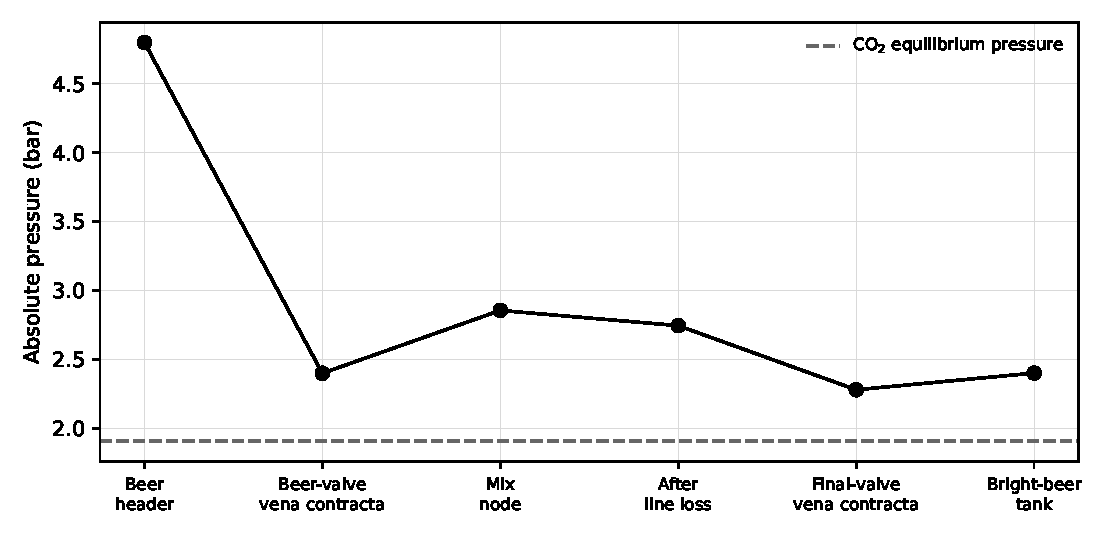
\includegraphics[width=0.92\textwidth]{pressure_profile.pdf}
\caption{Absolute pressure along the beer path at the lager steady point. The dashed line is the carbon-dioxide equilibrium pressure of the finished beer.}
\label{fig:pressure}
\end{figure}

\begin{figure}[htbp]
\centering
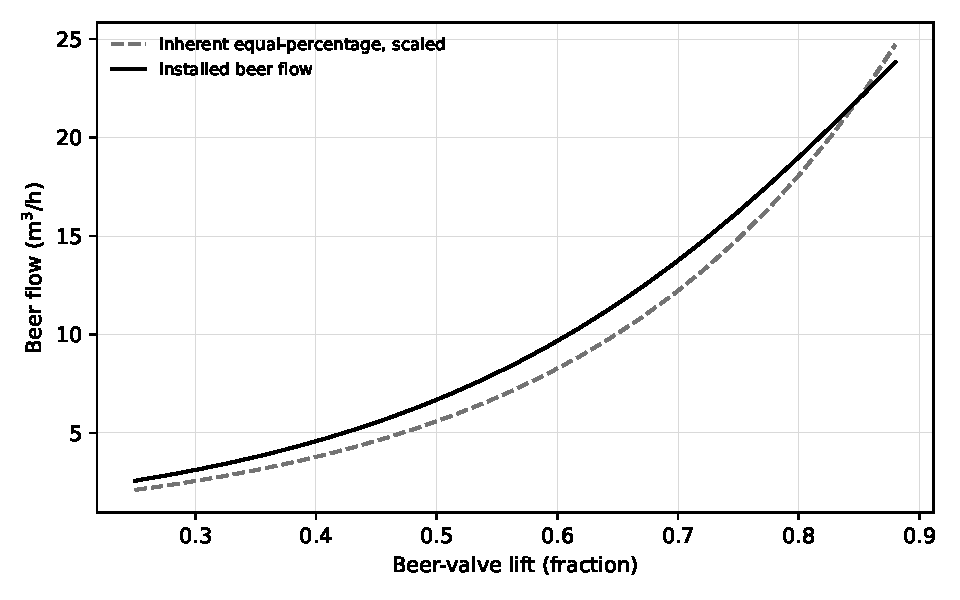
\includegraphics[width=0.78\textwidth]{installed_characteristic.pdf}
\caption{Inherent equal-percentage capacity, scaled to the installed beer flow at lift $0.85$, and the beer flow the network passes with the water and final valves fixed.}
\label{fig:char}
\end{figure}

The gain matrix and the relative-gain array are Table~\ref{tab:rga}, already interpreted in \eqref{eq:G} and \eqref{eq:RGAnum}. The estimation use of that table is practical. Decentralised loops are a fair baseline at this point, so a later improvement has to come from the transient, from the constraint, or from the model, not from a pathological pairing.

\subsection{Commissioning estimates}

Table~\ref{tab:est} is the result of Algorithm~\ref{alg:twin}. The three capacities are recovered to a tenth of a percent, with standard errors of $0.08$, $0.01$ and $0.12$ cubic metres per hour. The header bias is recovered as \SI{0.098}{bar} against \SI{0.100}{bar}, with a standard error of \SI{0.006}{bar}. The solubility scale is \SI{0.930}{} against \SI{0.930}{}. The contraction estimated from \eqref{eq:gammahat} is $1.187\times 10^{-4}$ against $1.20\times 10^{-4}$. These are the parameters the grade change needs, and the campaign of twenty-eight noisy steady points is enough to get them.

Roughness and minor loss are the parameters the campaign cannot separate. The least-squares point drove roughness to several millimetres and the minor-loss coefficient to zero, with a standard error on the minor loss of order $10^{2}$. That point is not reported as a roughness of the pipe, because the standard error says it is not one. The effective resistance $C_L$ computed from the same point at $\mathrm{Re}=4\times 10^{4}$ is $18.37$ against a true value of $18.85$, an error of two and a half percent. The two bad parameters have traded off inside a sum that the pressure drop can see. The next campaign should estimate $C_L$ as a single positive parameter and should stop printing $\varepsilon$.

Figure~\ref{fig:parity} is the beer-flow parity of the nominal model and of the commissioned physical model. The nominal cloud is biased by the wrong capacity and the wrong header. The commissioned cloud lies on the diagonal, inside the \SI{0.03}{\cubic\metre\per\hour} noise that was added to the measurements. The held-out root-mean-square residual of the physical model is \SI{0.030}{\cubic\metre\per\hour}. After the residual network is trained, the same held-out residual is \SI{0.037}{\cubic\metre\per\hour}. The network has learned noise. The gate of Algorithm~\ref{alg:twin} therefore publishes $\Delta Q = 0$, and every closed-loop trace in this chapter that is labelled with the twin is using the calibrated physical parameters only. This is the result anticipated in Section~\ref{sec:twin}. A physics-informed residual is part of the design, and on this skid it is correctly left unused. \citet{kadlec2009} describe the same decision as the maintenance step of a soft sensor: a block that does not improve held-out data is taken out of service.

\begin{figure}[htbp]
\centering
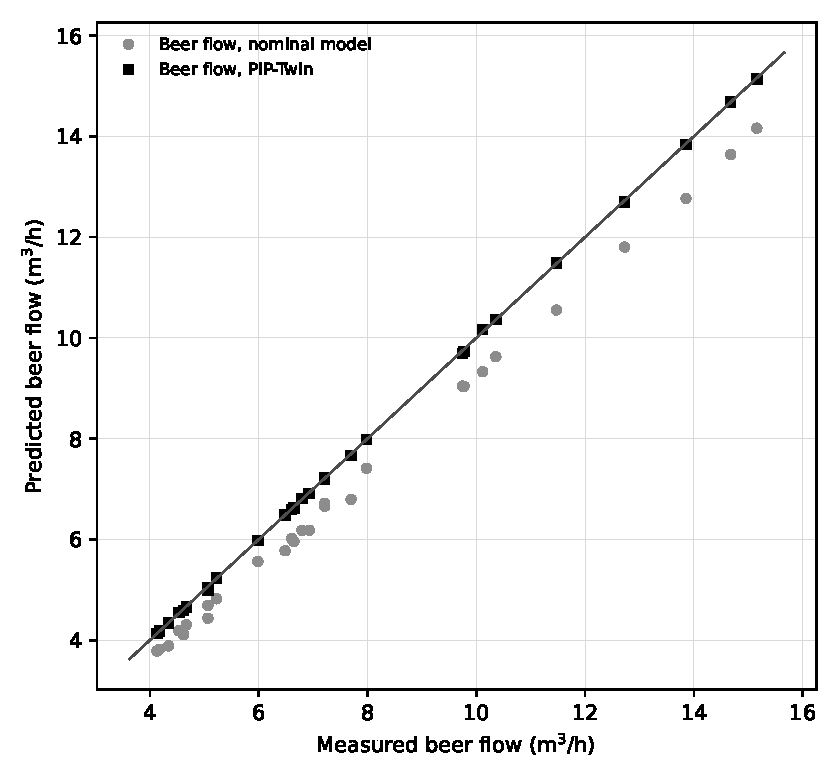
\includegraphics[width=0.72\textwidth]{parity_flow.pdf}
\caption{Beer flow predicted by the nominal model and by the commissioned twin, against the measured beer flow on the commissioning points.}
\label{fig:parity}
\end{figure}

\subsection{Grade change}
\label{sec:s1}

Figure~\ref{fig:s1q} is original extract, alcohol and carbon dioxide through the grade change. Figure~\ref{fig:s1v} is the three lifts. Figure~\ref{fig:bars} collects the extract integrals of all three scenarios. The numbers are the first block of Table~\ref{tab:kpi}.

The ratio station and the predictive controller on the nominal model finish with almost the same extract integral, \SI{31.3}{\degree}P$\cdot$s and \SI{32.3}{\degree}P$\cdot$s. The nominal predictive controller leaves a tail error of \SI{0.19}{\degree}P. Its model, given the wrong capacity and the biased header, believes a lift that is not the lift the plant needs, and re-optimisation from a measured state does not remove an error that the model explains away. The ratio station, integrating measured flow, brings the mean tail error down to \SI{0.02}{\degree}P, but it spends a valve travel of $7.1$ lift-units getting there and its flow integral is \SI{107}{(\cubic\metre\per\hour)\cdot s}, against \SI{51}{} to \SI{68}{} for the predictive controllers. The strict settling test, every sample inside \SI{0.05}{\degree}P for the rest of the run, is not met by either of those two controllers inside the \SI{130}{\second} that remain.

The predictive controller on the commissioned twin meets the strict test at \SI{16}{\second}. The first applied move sits on the rate limit of $0.16$ lift on all three valves: beer flow falls to about \SI{6.4}{\cubic\metre\per\hour} and water flow rises to about \SI{10.2}{\cubic\metre\per\hour}, so the inlet is lighter than the light brand and the extract falls faster than $\mathrm{e}^{-t/\tau}$. Four seconds after the upset the error is \SI{0.87}{\degree}P, against \SI{1.46}{\degree}P for a residence-time decay of the same step. The tail errors, once the flows have returned near \SI{11.5}{\cubic\metre\per\hour} and \SI{8.5}{\cubic\metre\per\hour}, are \SI{0.012}{\degree}P, \SI{0.005}{\percent} by volume and \SI{0.001}{\gram\per\litre}. The extract integral falls from about \SI{32}{\degree}P$\cdot$s to \SI{10.7}{\degree}P$\cdot$s. Carbon dioxide falls from \SI{11.8}{} and \SI{8.1}{} to \SI{2.1}{\gram\per\litre}$\cdot$s. The minimum mix-pressure margin stays at \SI{0.95}{bar}, and no vena contracta crosses equilibrium. Dissolved oxygen stays near \SI{9.7}{ppb}. The maximum extract excursion is \SI{1.92}{\degree}P, which is the size of the setpoint step itself, recorded at the sample the step is applied. Section~\ref{sec:firstsample} gives the lifts.

Table~\ref{tab:s1trace} is that same trajectory at the control samples, taken from the commissioned run. The steady light-brand flows are about \SI{11.6}{\cubic\metre\per\hour} of beer and \SI{8.4}{\cubic\metre\per\hour} of water. The first applied command does not go there. It cuts the beer flow by more than half and raises the water flow above the new steady value, and every lift moves by the legal maximum of $0.16$. The extract error drops from \SI{1.92}{\degree}P to \SI{0.87}{\degree}P in that one sample. The sample at \SI{9}{\second} is the clumsy one: product flow falls to \SI{13.2}{\cubic\metre\per\hour} while the ratio is being put back, and the extract almost stops moving. By \SI{16}{\second} the error is \SI{0.04}{\degree}P and the flows are within about \SI{1}{\cubic\metre\per\hour} of the light-brand steady state. The dose, which is \SI{7.5}{\gram\per\second} on the lager, is above \SI{9}{\gram\per\second} throughout, because the light brand contains more uncarbonated water even after the overshoot has been removed.

\begin{table}[htbp]
\centering
\caption{Commissioned grade change, at the control samples after the upset. Flows are cubic metres per hour and the dose is grams per second.}
\label{tab:s1trace}
\begin{tabular}{rrrrrr}\toprule
Time (s) & $Q_h$ & $Q_w$ & $Q_f$ & Dose & Extract error ($^\circ$P) \\\midrule
0 & 13.8 & 6.1 & 19.9 & 7.7 & $+1.92$ \\
1 & 6.4 & 10.2 & 16.6 & 9.4 & $+1.64$ \\
5 & 9.0 & 10.7 & 19.7 & 11.6 & $+0.68$ \\
9 & 7.7 & 5.6 & 13.2 & 9.3 & $+0.17$ \\
13 & 11.7 & 9.2 & 20.9 & 10.7 & $+0.12$ \\
16 & 11.7 & 9.2 & 20.9 & 10.0 & $+0.04$ \\
21 & 11.6 & 8.4 & 20.0 & 10.1 & $-0.01$ \\
\bottomrule\end{tabular}
\end{table}

The product-flow integral on this path, accumulated in the same way as the extract integral, is \SI{51}{(\cubic\metre\per\hour)\cdot s}. A move that had gone straight to the steady light-brand lifts would have charged much less flow error and left the vessel to forget the lager at $\tau=\SI{14.4}{\second}$. At that rate the error at \SI{16}{\second} would still be about \SI{0.63}{\degree}P, and the strict band would be missed. The \SI{51}{} is the price of not missing it. It is smaller than the ratio station's flow integral of \SI{107}{(\cubic\metre\per\hour)\cdot s}, and it is paid once, at the start, rather than as a reversal hunt across the rest of the run.

The grade-change estimate is therefore not that predictive control beats ratio control. On the nominal model it does not, for extract. The estimate is that predictive control on the commissioned twin brings a feasible brand change inside the extract tolerance in \SI{16}{\second} by spending the rate limit once, and that the same predictive control on the uncommissioned model does not. The first technology needs the second.

\begin{figure}[htbp]
\centering
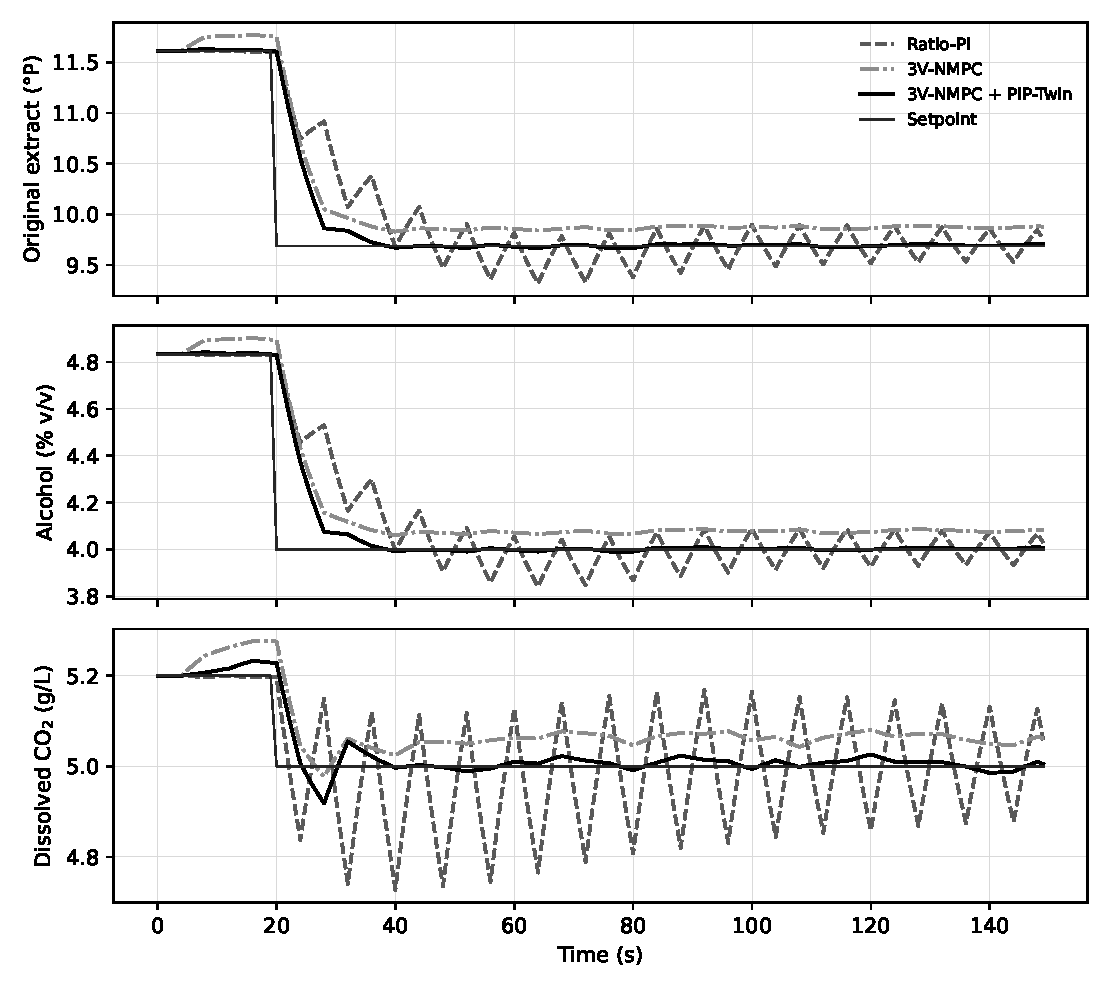
\includegraphics[width=0.92\textwidth]{s1_quality.pdf}
\caption{Grade change from the lager to the light brand at $t=\SI{20}{\second}$. The thin line is the setpoint.}
\label{fig:s1q}
\end{figure}

\begin{figure}[htbp]
\centering
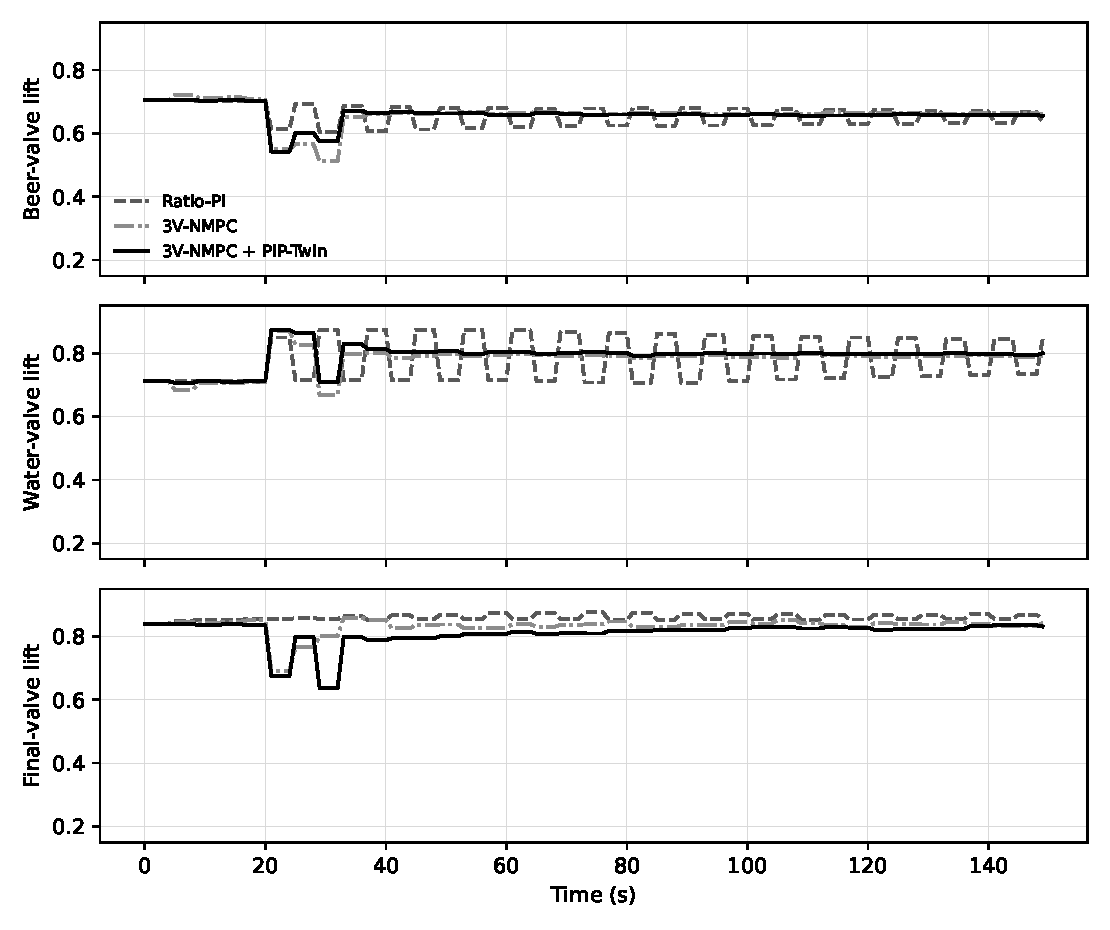
\includegraphics[width=0.92\textwidth]{s1_valves.pdf}
\caption{Valve lifts during the grade change. The ratio station continues to move after the predictive controllers have stopped.}
\label{fig:s1v}
\end{figure}

\begin{figure}[htbp]
\centering
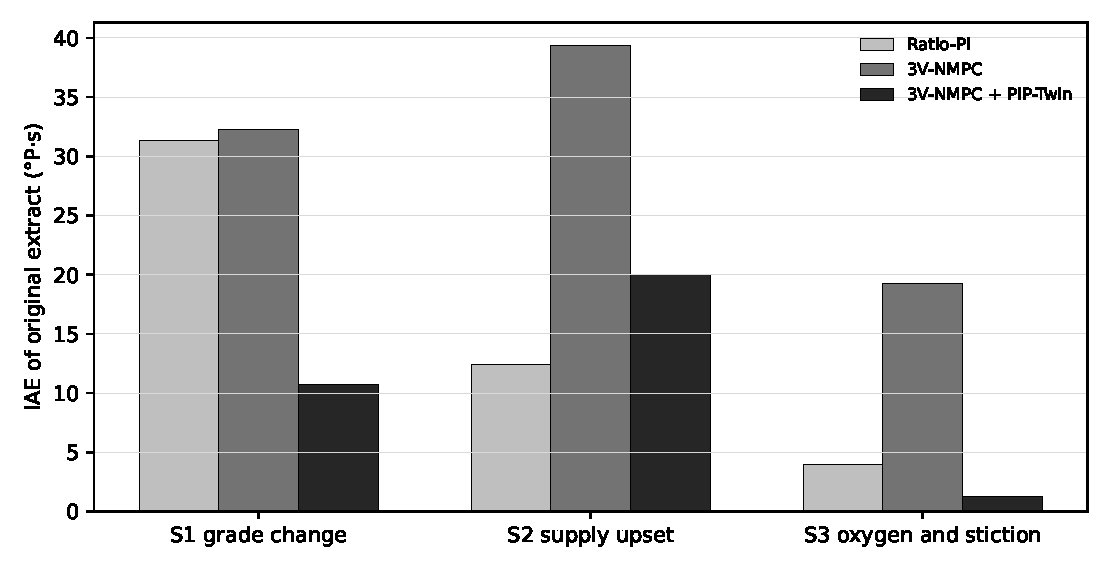
\includegraphics[width=0.92\textwidth]{iae_bars.pdf}
\caption{Integral absolute error of original extract from the upset to the end of each run.}
\label{fig:bars}
\end{figure}

\subsection{A mother beer that makes the brand infeasible}
\label{sec:s2}

After the supply upset the mother beer is $A_w=\SI{5.15}{\percent}$ and $E_r=\SI{6.55}{\percent}$. Its original extract, by \eqref{eq:balling}, is \SI{16.297}{\degree}P, almost unchanged. Its alcohol is \SI{6.617}{\percent} by volume rather than \SI{6.923}{\percent}. A one-dimensional search in $w$ on the plant density gives the two pure compromises and the weighted one. The mass fraction that restores the lager extract is $w=0.702$, and the alcohol there is \SI{4.626}{\percent} by volume, short by \SI{0.207}{\percent}. The mass fraction that restores the lager alcohol is $w=0.733$, and the original extract there is \SI{12.106}{\degree}P, high by \SI{0.493}{\degree}P. The mass fraction that minimises \eqref{eq:stage} without the flow and pressure terms is $w=0.712$, at \SI{11.780}{\degree}P and \SI{4.696}{\percent} by volume. In tolerance units that point costs about $32$. The extract-only point costs about $48$. The alcohol-only point costs about $97$. The weighted optimum sits closer to the extract target because a half-degree extract miss is more tolerances than a fifth of a percent of alcohol, and it does not sit on the extract target, because giving up all of the alcohol is still expensive.

Figure~\ref{fig:s2q} and the second block of Table~\ref{tab:kpi} are what the three controllers do with that geometry. The ratio station's tail is $+\SI{0.091}{\degree}P$ and $-\SI{0.169}{\percent}$ by volume. Its integral on extract has pulled it toward the extract-only point. The nominal predictive controller's tail is $+\SI{0.303}{\degree}P$ and $-\SI{0.080}{\percent}$ by volume: the biased model has chased alcohol and missed the weighted point. The commissioned predictive controller's tail is $+\SI{0.164}{\degree}P$ and $-\SI{0.138}{\percent}$ by volume, which is \SI{11.777}{\degree}P and \SI{4.695}{\percent} by volume, against the calculated optimum of \SI{11.780}{\degree}P and \SI{4.696}{\percent}. The match is inside the noise of the tail average.

No controller records a settling time inside \SI{0.05}{\degree}P, because the weighted optimum itself lies \SI{0.17}{\degree}P off the setpoint. A settling test written on a single setpoint is the wrong test for an infeasible brand. The right test is the distance to the weighted point, and on that test the commissioned controller has arrived. It also holds carbon dioxide to an integral of \SI{1.27}{\gram\per\litre}$\cdot$s against \SI{2.83}{} and \SI{5.06}{}, and product flow to \SI{10.2}{(\cubic\metre\per\hour)\cdot s} against \SI{30.5}{} and \SI{45.2}{}. The header step of \SI{0.45}{bar} is absorbed without a vena-contracta violation. The minimum margins remain above \SI{0.86}{bar}.

The estimate from this upset is that a calibrated predictive controller states the compromise the tolerances asked for, and that a ratio station with an extract integral states a different compromise without saying so. Neither technology creates a second ratio. The alcohol that the fermentation did not produce is not in the skid.

\begin{figure}[htbp]
\centering
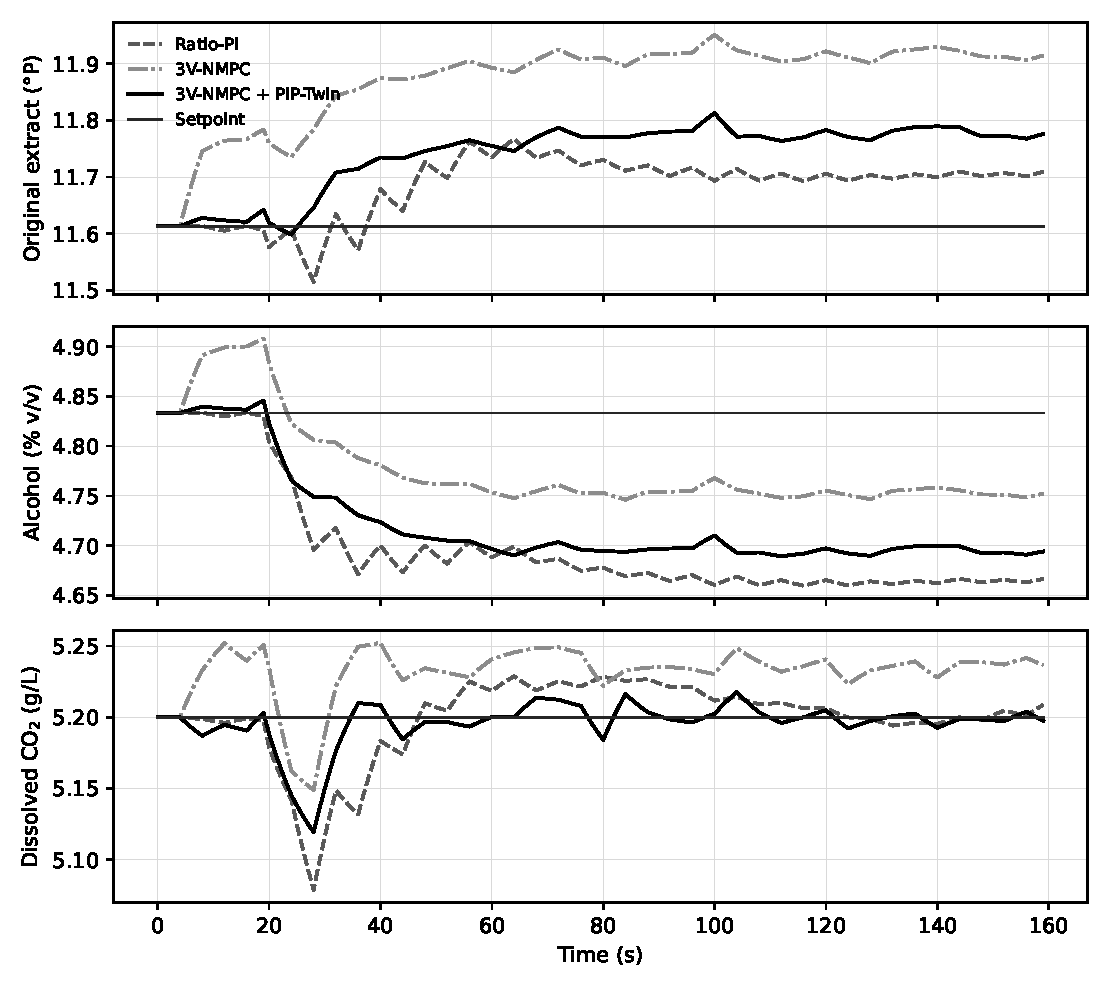
\includegraphics[width=0.92\textwidth]{s2_quality.pdf}
\caption{Supply upset at $t=\SI{20}{\second}$: beer-header pressure down by \SI{0.45}{bar}, mother beer less attenuated. Setpoints are unchanged and are not jointly feasible.}
\label{fig:s2q}
\end{figure}

\subsection{Oxygen and a sticky water valve}
\label{sec:s3}

The oxygen balance at $w=0.70$ with \SI{85}{ppb} in the water and \SI{8}{ppb} in the beer is
\begin{equation}
c_{\mathrm{DO}}
\approx
0.697\times 8 + 0.303\times 85
=
\SI{31.3}{ppb},
\end{equation}
using the volumetric water fraction $6.06/20$. Table~\ref{tab:kpi} reports a maximum dissolved oxygen between \SI{31.2}{ppb} and \SI{31.4}{ppb} for every controller. Figure~\ref{fig:s3q} shows the quality channels; the oxygen itself is the number in the table rather than a fourth trace, because the three traces would overlap. No valve motion removed the oxygen, and no valve motion added a flashing pickup, because the margin stayed above \SI{0.86}{bar}. The alarm at \SI{30}{ppb} is the correct output of the estimator. A controller that moved the water valve to chase a lower oxygen would have left the brand. The phase logic of Section~\ref{sec:build} holds the brand or switches the water source. It does not retune $w$.

The sticky valve is a different estimate. The ratio station's extract integral is \SI{4.0}{\degree}P$\cdot$s and its strict settling time is \SI{107}{\second}, with a tail error of \SI{0.040}{\degree}P. The nominal predictive controller, wrong gain plus an unknown deadband, is worse: an integral of \SI{19.3}{\degree}P$\cdot$s and a tail of \SI{0.144}{\degree}P. The commissioned controller, with the inverse \eqref{eq:invstick} after the eight-second detection delay, keeps the maximum extract error at \SI{0.035}{\degree}P and is therefore inside the settling band from the start of the upset. Its integral is \SI{1.3}{\degree}P$\cdot$s. Valve travel is higher than the ratio station's, $0.63$ against $0.20$, because the inverse takes a deliberate step through the deadband instead of waiting for an integral to creep across it. The beer moves less than the valve does.

The estimate from this upset has two sentences. Dissolved oxygen that arrives in the water is observed and is not a control degree of freedom. Stiction that is estimated and inverted stays inside the extract tolerance; the same predictive controller without that estimate, and with a biased capacity, is the worst of the three stations. Deploying the first technology without the second is not a conservative choice. On this upset it is the expensive one.

\begin{figure}[htbp]
\centering
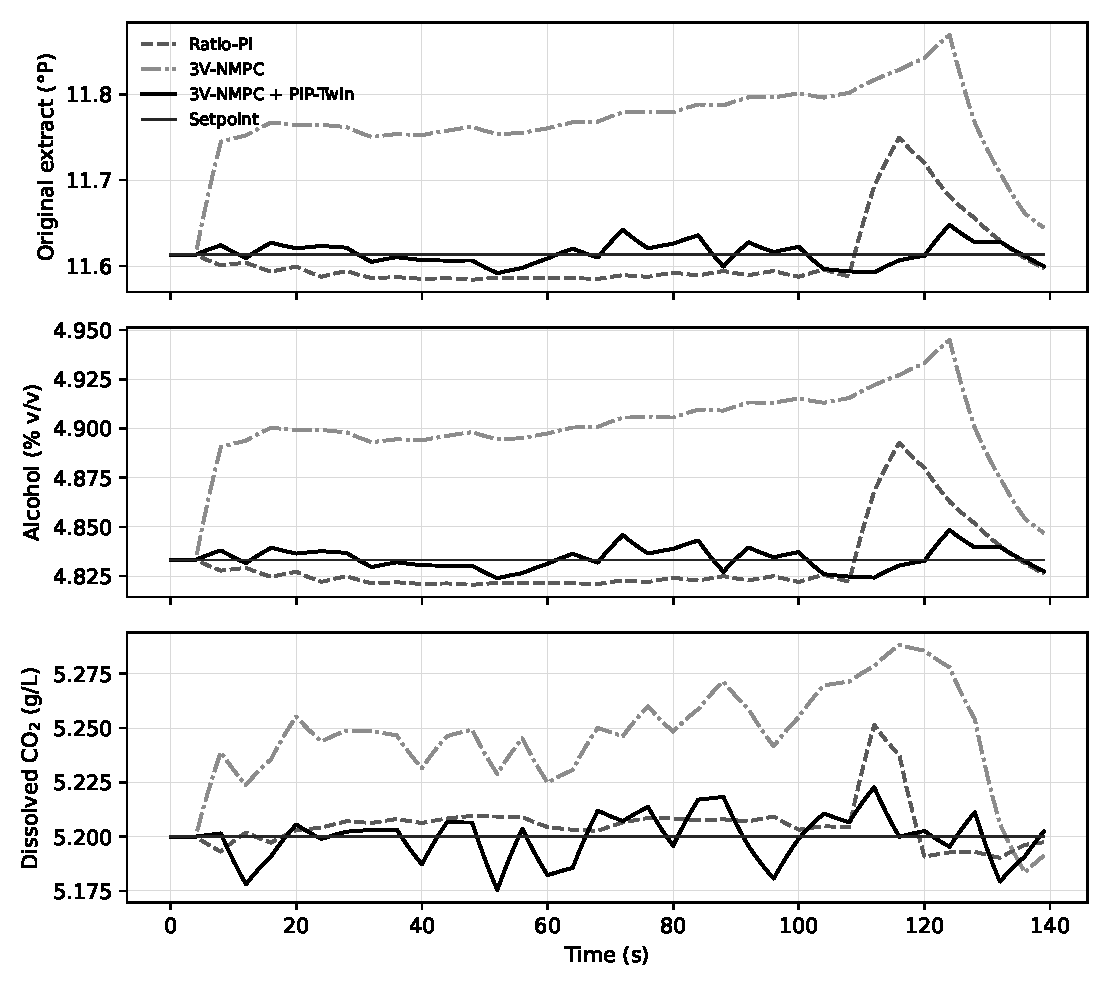
\includegraphics[width=0.92\textwidth]{s3_quality.pdf}
\caption{Dilution-water oxygen raised to \SI{85}{ppb} and a water-valve deadband of $0.03$ lift, from $t=\SI{20}{\second}$. Extract and alcohol stay near the lager setpoint only for the commissioned controller.}
\label{fig:s3q}
\end{figure}

\subsection{Pressure drop, station by station}

The hand solution of Section~\ref{sec:hand} can be read as a commissioning sheet. At the lager point the beer header is \SI{4.80}{bar}. The beer valve consumes \SI{1.945}{bar}. The mix node is \SI{2.855}{bar}. The line, with $C_L=18.85$, consumes about \SI{0.11}{bar}. The final valve consumes about \SI{0.34}{bar} and delivers the beer to a tank at \SI{2.40}{bar}. The throat of that valve is not at \SI{2.40}{bar}. It is at \SI{2.28}{bar}, because $F_L=0.86$ puts the vena contracta \SI{0.46}{bar} below the upstream pressure of the valve and the recovery does not give all of that drop back before the throat. Equilibrium is \SI{1.905}{bar}. The sheet therefore has two margins, \SI{0.95}{bar} at the transmitter and \SI{0.37}{bar} at the throat, and only the second one is the flash margin.

A pressure survey that records the transmitter and not the throat will accept a final valve with a poor recovery factor. The controller cannot see the throat either. It computes it from $F_L$, which is a number from the valve data sheet \citep{fisher2005,iec60534}, and from the pressures it can measure. Commissioning checks the computation by confirming that the measured mix pressure, the measured tank pressure and the measured flow are consistent with the $C_L$ and the $K_{v,f}$ in Table~\ref{tab:est}. They are, to the standard errors in that table. A discrepancy larger than those standard errors is a fouled mixer or a wrong recovery factor, and it is a reason to reopen the gate on the residual network rather than a reason to detune the brand.

The velocities that go with this sheet are \SI{1.134}{\metre\per\second} on the beer, \SI{0.762}{\metre\per\second} on the water and \SI{1.078}{\metre\per\second} on the product. All three are in the turbulent hygienic range. The water line is the slowest, which is one reason a sticky water valve is the fault worth injecting: a valve that spends its life at a modest opening and a modest velocity is the valve whose stem is most likely to sit. The beer valve, at a higher opening and a higher gain, shows a stick as a flow error immediately. The water valve can hide a deadband of $0.03$ lift inside a flow change of less than one cubic metre per hour until the grade change asks it to move.

\subsection{What was estimated, and what a brewery still has to measure}

The parameter estimation is Table~\ref{tab:est}: capacities and header bias to a small fraction of their values, solubility scale and contraction from their own one-point experiments, line resistance as a sum and not as a roughness. The quality estimation is Table~\ref{tab:kpi} together with the weighted point of Section~\ref{sec:s2}. On a feasible grade change the commissioned controller is inside \SI{0.05}{\degree}P in one residence time, and the uncommissioned predictive controller is not better than ratio control. On an infeasible mother beer the commissioned controller sits on the tolerance-weighted compromise to three decimal places of the steady calculation. On a sticky water valve it holds the brand, and on oxygenated dilution water it reports an alarm that every controller's product confirms at \SI{31}{ppb}.

Several limits are part of the estimate rather than footnotes under it. The plant and the twin share the same equation structure. A real trim that is not equal-percentage, or a mixer that is not a single volume, would open the residual-network gate and should be tested by repeating the hold-out on plant step tests before the gate is trusted. The pressure solver and the short sequential-quadratic program are not a certified real-time iteration; the timing result is that a \SI{12}{\second} horizon of this size solves in well under the \SI{4}{\second} sample on a desktop, which is necessary and not sufficient for an embedded controller. The terminal constraint that would support a stability argument was not imposed. Sensor faults were noise and one bias, not a failed meter. The bright-tank pressure was a boundary that had already been raised high enough to make the vena contracta feasible. A cellar that cannot provide that pressure has a different problem, and the controller will correctly spend flow to protect $p_{\mathrm{eq}}$ only inside the limits of the headers it is given.

Foam, yeast stress and the flavour match between a high-gravity beer and a sales-gravity beer remain the fermentation questions reviewed by \citet{stewart2010}, \citet{gibson2007} and \citet{bamforth2009}. The skid does not answer them. What it can answer, and what this estimation measured, is whether the beer that dilution is capable of making is the beer that leaves the final valve. With the three lifts and the carbon-dioxide dose chosen by the predictive controller, and with the model of that controller commissioned by the twin, the feasible brand is inside the extract tolerance sixteen seconds after the change, the infeasible brand leaves at the compromise the tolerances define, and the oxygen that no valve can remove is reported rather than stirred.
